\section{Technical Approach}
In this section, I present the concept to use mobility data, behavior data and pandemic data to calibrate and test a networked SEIR model. The theoretical concept of the networked SEIR model is introduced in \autoref{ssec:networkedSEIRModel}, which is followed by implementation specifics in \autoref{ssec:implementation}.

\subsection{Networked SEIR model}\label{ssec:networkedSEIRModel}

The idea of a networked SEIR model builds on the widely employed concept of epidemic models, that divide populations into compartments, whose relations are described as a set of differential equations. The basic SIR model is extended to the SEIR as introduced by \cite{aronSeasonalityPerioddoublingBifurcations1984} to account for epidemic scenarios in which humans are not immediately infectious after contact but have a static incubation period in becoming so. Therefore it is applicable to analyze virus-induced epidemics like COVID-19. Additional to the standard SEIR model, two sets of spread rates $\beta$ are introduced in equations 2 and 3 of \cite{vrabacCapturingEffectsTransportation2020}. While $\beta_{I1}, \beta_{I2}, \beta_{I3}$ relate to the standard SEIR model spread from infectious to exposed compartments, the new set of spread rates $\beta_{E1}, \beta_{E2}, \beta_{E3}$ allow to model the spread from exposed compartments to other exposed compartments.

The networked SEIR model from \cite{vrabacCapturingEffectsTransportation2020} takes this idea even further, in that it aims to identify spread parameters for a population divided into many subpopulations, which itself are divided into the SEIR compartments. Each of these subpopulations is modeled to influence the compartments of geographically adjacent regions by parameter $A1$, their own compartments by means of community spreading with parameter $A2$ and due to the travel behavior of humans inscribed by $A3$. $A1$, $A2$ and $A3$ are all so-called adjacency matrices, which model the strength of relationship between network entities. Entities relate to political counties in this analysis.

\subsubsection{Identifying the networked SEIR model parameters}\label{ssec:identifyNetworkedSEIR}
The identification of the networked SEIR model can be expressed as an optimization problem, that results from discretization of the system of continuous partial differential equations. The following brief discussion is based on the paper and prototypic implementation in \cite{vrabacCapturingEffectsTransportation2020}.

The optimization problem revolves around finding spread parameters that describe the pandemic spread across  a number of counties \eqref{eq:1}, for a number of time steps \eqref{eq:2} by using pandemic data with the sample rate $h$, which equals 1 in most scenarios.

% subequations?
\begin{equation}
\begin{aligned}
	m &= N_{counties} = const.% \label{eq:1}
\\ 
	n &= N_{timesteps} = const.% \label{eq:2}
\\
	j &\in \{1, 2, ..., n-1\}
\end{aligned}
\end{equation}

For each of these counties and days of analysis, a difference equation for the compartments exposed, infectious and removed describes the rate of change. The difference equations are expressed in vector form to simply the optimization problem, hence the input data matrices $E_{(n\times m)}$, $I_{(n\times m)}$ and $R_{(n\times m)}$ are reshaped\footnote{Notation refers to the MATLAB implementation \url{https://www.mathworks.com/help/matlab/ref/reshape.html}} as vectors $e$, $i$ and $r$. As we intend to identify one set of spread parameters common to all regions under analysis, the input case data matrices are expected to be normalized using each region's number of residents.

\begin{align}
\startsubequation\tagsubequation\label{eq:4a}
	e &= reshape(E_{(n\times m)}^T, n*m, 1)
\\
\tagsubequation\label{eq:4b}
	i &= reshape(I_{(n\times m)}^T, n*m, 1)
\\
\tagsubequation\label{eq:4c}
	r &= reshape(R_{(n\times m)}^T, n*m, 1)
\\
\tagsubequation\label{eq:4d}
	\Delta_e &= e_{(n+1:end)} - e_{(1:(m-1)*n)}
\\
\tagsubequation\label{eq:4e}
	\Delta_i &= i_{(n+1:end)} - i_{(1:(m-1)*n)}
\\
\tagsubequation\label{eq:4f}
	\Delta_r &= r_{(n+1:end)} - r_{(1:(m-1)*n)}
\\
	\Delta &= [\Delta_e ; \Delta_i ; \Delta_r]
\end{align}

While the adjacency matrices $A1$ (models adjacent county spread) and $A2$ (models intra-county spread) are static by nature, $A3$ (models mobility-driven spread) introduces time-dependent strength of connectedness, e.g. number of vehicles moving--and hence changes with each iteration $j$. To further consider the time-dependent mobility behavior of the population and policy behavior of the government, the parameters $\psi_{1_j}$, $\psi_{2_j}$ and $\psi_{3_j}$ are introduced. Depending on the data set, these can be either scalar values representing similar behavior in all counties or diagonal matrices, wherein each element of the diagonal describes the mobility behavior and policy information of one region under analysis. Extending the works of Vrabac et al., this work determines the parameters $\psi$ in a data-driven approach in \autoref{ssec:implementation}.

\begin{align}
\startsubequation\tagsubequation\label{eq:6a}
    A1_{s_j} &= \psi_{1_j} A1
\\
\tagsubequation\label{eq:6b}
    A2_{s_j} &= \psi_{2_j} A2
\\
\tagsubequation\label{eq:6c}
    A3_{s_j} &= \psi_{3_j} A3_j
\end{align}

The daily levels of each compartment \eqref{eq:4a}, \eqref{eq:4b} and \eqref{eq:4c} are then used to determine the discretized, time-dependent version of the networked SEIR model as described by \eqref{eq:8}. The networked SEIR model is then parametrized using the parameter vector $[\beta_{E1}, \beta_{E2}, \beta_{E3}, \beta_{I1}, \beta_{I2}, \beta_{I3}, \sigma, \gamma]$. These parameters are identified based on the optimization problem stated as \eqref{eq:9}, which is the minimum square normed difference of the parametrized networked SEIR model compartments and the actual daily difference of compartments given by the input data.

\begin{align}
\startsubequation\tagsubequation\label{eq:7a}
	S_j &= \mathds{1} - diag(e_j + i_j + r_j)
\\
\tagsubequation\label{eq:7b}
	e_j &= e_{(n*(j-1)+1:n*j)}
\\
\tagsubequation\label{eq:7c}
	i_j &= i_{(n*(j-1)+1:n*j)}
\\
\tagsubequation\label{eq:7d}
	r_j &= r_{(n*(j-1)+1:n*j)}
\\
\tagsubequation\label{eq:7e}
\begin{split}
	\delta_{e_j} &= h [S_j A1_{s_j} e_j, S_j A2_{s_j} e_j, S_j A3_{s_j} e_j,
	\\
	&\quad S_j A1_{s_j} i_j, S_j A2_{s_j} i_j, S_j A3_{s_j} i_j, -e_j, 0]
\end{split}
\\
\tagsubequation\label{eq:7f}
	\delta_{i_j} &= h [0, 0, 0, 0, 0, 0, e_j, i_j]
\\
\tagsubequation\label{eq:7g}
	\delta_{r_j} &= h [0, 0, 0, 0, 0, 0, 0, i_j]
\\
	\delta &= [\delta_e; \delta_i; \delta_r] \label{eq:8}
\\
	\begin{split}
		&[\beta_{E1}^*, \beta_{E2}^*, \beta_{E3}^*, \beta_{I1}^*, \beta_{I2}^*, \beta_{I3}^*, \sigma^*, \gamma^*] =
		\\
		&\argmin_{\beta_{E1}, \beta_{E2}, \beta_{E3}, \beta_{I1}, \beta_{I2}, \beta_{I3}, \sigma, \gamma}
		\\
		&\{\lVert \delta [\beta_{E1}, \beta_{E2}, \beta_{E3}, \beta_{I1}, \beta_{I2}, \beta_{I3}, \sigma, \gamma]^T - \Delta\rVert\} \label{eq:9}
	\end{split}
\end{align}

To ensure plausible results, the optimization problem is constrained. Firstly, the spread parameters are required to be non-negative \eqref{eq:10a}. Secondly, the incubation rate $\sigma$ is upper-bounded by a static time delay introduced to estimate the exposed compartment \eqref{eq:10b}. This delay shifts the data of the infectious compartment data - as derived from government agency data - by $\Delta_{t_{preExposed}}$ days into the past. Thirdly, the cure rate $\gamma$ is upper-bounded \eqref{eq:10c}. Lastly, the combined spread rates described by the parameters $\beta$ and the adjacency matrices $A$ are upper-bounded by the inverse of the sample rate $h$ for each time step $j$ and region $k \in \{1, 2, ..., m\}$ \eqref{eq:10d}.

\begin{align}
\startsubequation\tagsubequation\label{eq:10a}
	\beta_{E1}, \beta_{E2}, \beta_{E3}, \beta_{I1}, \beta_{I2}, \beta_{I3}, \sigma, \gamma &>= 0
\\
\tagsubequation\label{eq:10b}
	\sigma &<= 1/\Delta_{t_{preExposed}}
\\
\tagsubequation\label{eq:10c}
	\gamma &<= 1
\\
\tagsubequation\label{eq:10d}
\begin{split}
	\vert A1_{s_{j_{(k, 1:m)}}} \vert (\beta_{E1} + \beta_{I1}) &+ \vert A2_{s_{j_{(k, 1:m)}}} \vert (\beta_{E2} + \beta_{I2})
	\\
	+ \vert A3_{s_{j_{(k, 1:m)}}} \vert (\beta_{E3} + \beta_{I3}) &<= 1/h
\end{split}
\end{align}

\subsubsection{Simulating the networked SEIR Model}

Based on the parametrized networked SEIR model, we can calculate the pandemic spread per compartment, region and day. The entry point for the simulation is the set of initial conditions $\{s_{t0}, i_{t0}, e_{t0}, r_{t0}\}$, which describe the initial pandemic levels of each region, and the parameter vector $[\beta_{E1}, \beta_{E2}, \beta_{E3}, \beta_{I1}, \beta_{I2}, \beta_{I3}, \sigma, \gamma]$. Using \eqref{eq:6a}, \eqref{eq:6b} and \eqref{eq:6c} an iterative problem to determine the pandemic levels is stated by the following set of equations:

\begin{align}
\startsubequation\tagsubequation\label{eq:11a}
	S_j &= \mathds{1} - diag(e_j + i_j + r_j)
\\
\tagsubequation\label{eq:11b}
\begin{split}
    e_{j+1} &= e_j + h (S_j (
    \\
    &(\beta_{E1} A1_{s_j} + \beta_{E2} A2_{s_j} + \beta_{E3} A3_{s_j}) e_j^T + 
    \\
    &(\beta_{I1} A1_{s_j} + \beta_{I2} A2_{s_j} + \beta_{I3} A3_{s_j}) i_j^T) - \sigma e_j^T)^T
\end{split}
\\
\tagsubequation\label{eq:11c}
	i_{j+1} &= i_j + h (\sigma e_j - \gamma i_j)
\\
\tagsubequation\label{eq:11d}
    r_{j+1} &= r_j + h (\gamma i_j)
\end{align}

\subsection{Implementation}\label{ssec:implementation}
To evaluate the aforementioned approach against German pandemic and mobility data, the networked SEIR model extending the works of Vrabac et al. and related data processing was implemented in MATLAB. This work covers the whole sequence from said data processing to model identification and simulation and is introduced in the following paragraphs. As the RKI data set \cite{robertkoch-institutrkiRKICOVID192021} provides data with a county resolution, this work implemented the networked SEIR model approach using German counties as regions under analysis.

\subsubsection{Data fusion pipeline}
To identify the networked SEIR model as described in \autoref{ssec:identifyNetworkedSEIR}, a number of different input data is required.

First and foremost, the COVID-19 pandemic information consisting of daily confirmed cases (confirmed as proxy for infectious, recovered and death as proxy for removed) is needed. This work relies on the official data set for Germany \cite{robertkoch-institutrkiRKICOVID192021}. The data is processed to yield the data matrices $E_{(n\times m)}$, $I_{(n\times m)}$ and $R_{(n\times m)}$, which are then normalized by the number of residents of each county, available from the geopolitical information provided by the government agency BKG \cite{Verwaltungsgebiete2500002020}.

Secondly, the three adjacency matrices have to be calculated. $A1$ can be derived by calculating all adjacent counties for each county using county shape information from \cite{Verwaltungsgebiete2500002020}. $A2$ is defined as a 2d eye matrix with both dimensions equaling the number of counties under analysis. The time-dependent $A3$ finally models mobility-driven spread and hence depends on mobility information. This work proposes a new method to calculate this matrix based on public transport schedule data \cite{delfie.v.OpenDataOPNV2021} and geopolitical data \cite{Verwaltungsgebiete2500002020}. The detailed approach is introduced in \autoref{ssec:transientAdjancencyMatrixCalculation}.

Lastly, the adjacency matrices have to be adjusted to actual, time-dependent behavior and policy of the population under analysis. This work implements the scaling based on behavior data, which is recovered from aggregated, anonymized mobile phone data. The matrices $A1, A2$ are hereby scaled using county resolution, total mobility behavior \cite{statistischesbundesamtdestatisVeranderungsrateMobilitatGgu2021}. As $A3$ models the public transport network, another data set that specifically recovered railway usage figures with nationwide resolution is applied for scaling \cite{statistischesbundesamtdestatisVerkehrsmittelImFernverkehr2021}. Though not part of this work, it is possible to introduce other auxiliary information for adjacency scaling. This notably includes information on COVID-19 policies \cite{haleGlobalPanelDatabase2021}, economic figures \cite{statistischesbundesamtdestatisKonjunkturindikatoren} and fine-grained mobility behavior \cite{COVID19CommunityMobility}.

The last data processing stage then determines the joint time range, for which pandemic information, transient adjacency and behavior information is available for subsequent SEIR model identification and simulation.

The relationship of data sets and processing stages is depicted in \autoref{img:flwData}.

\begin{figure}[hbtp]
\centering 
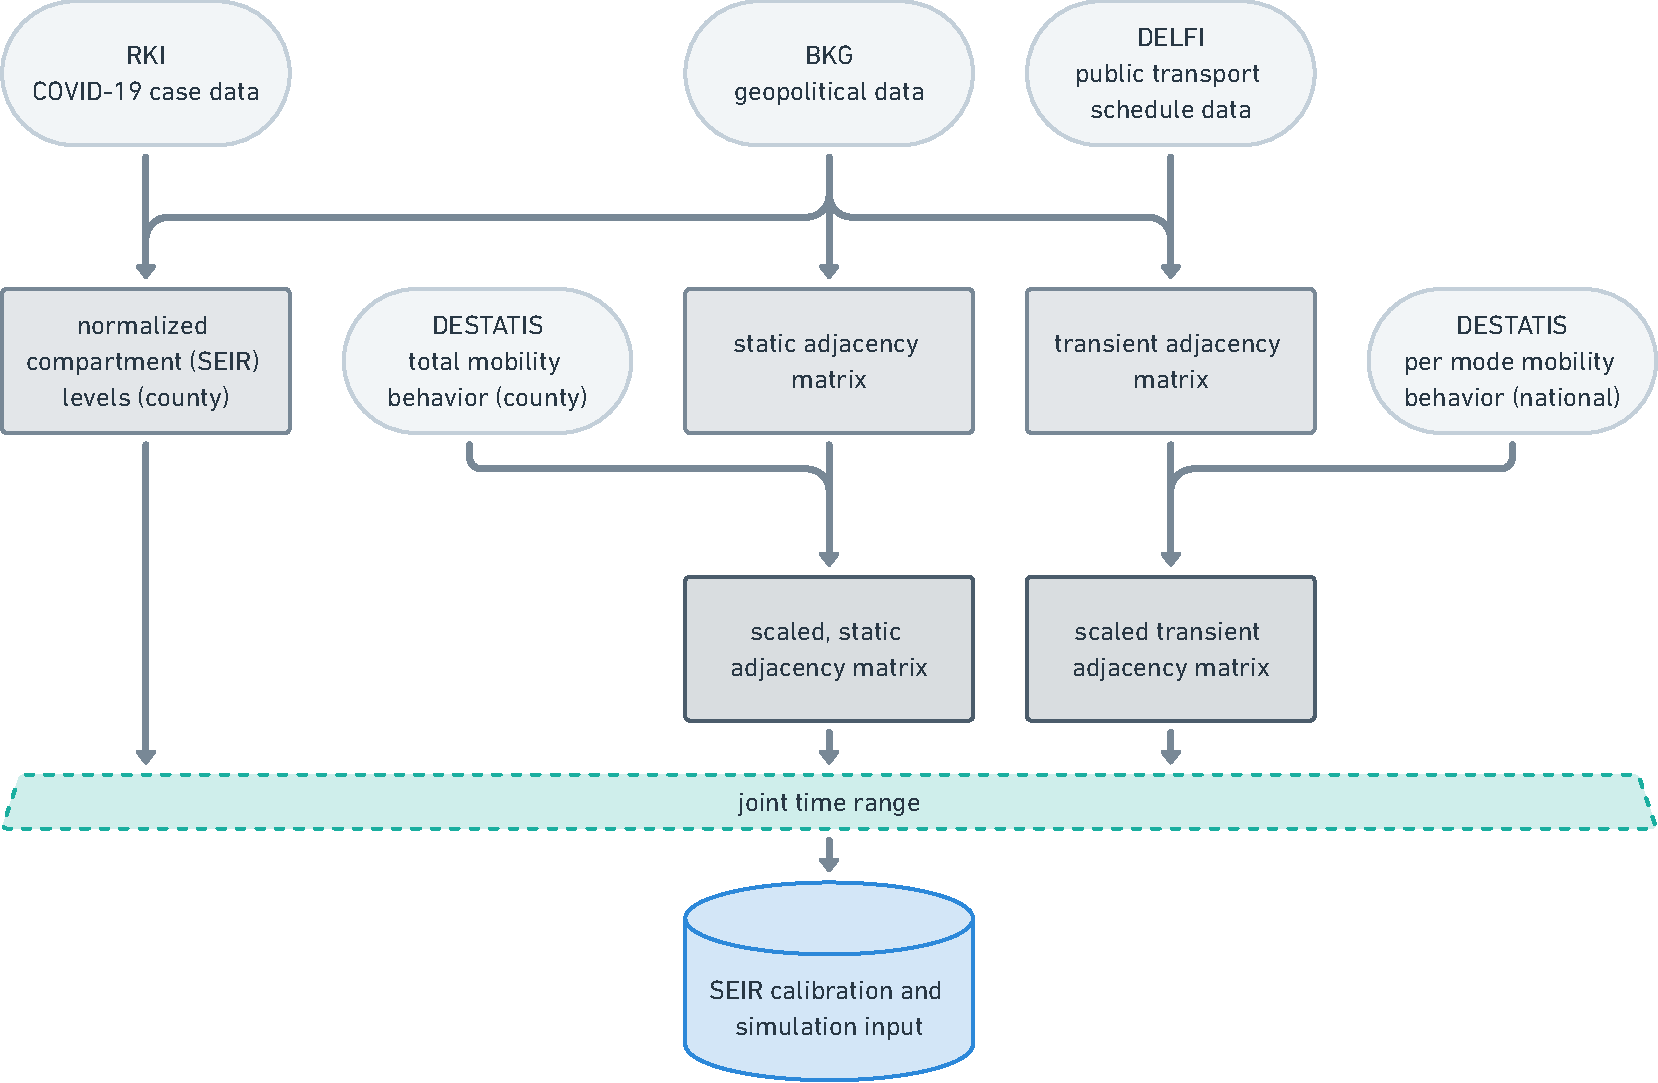
\includegraphics[width=\linewidth]{img/FP_data-pipeline.pdf}
\caption{Data processing pipeline}
  \label{img:flwData}
\end{figure}

\subsubsection{Transient adjacency matrix calculation}\label{ssec:transientAdjancencyMatrixCalculation}
The main body of work of this report is the new method to derive the transient adjacency matrix $A3$ from publicly available data in a programmatic way. The entry point for this calculation is the public transport schedule data collected by a project from DELFI e.V. \cite{delfie.v.OpenDataOPNV2021}. The data sets contain data on schedules of regional and national agencies operating across all of Germany. As the schedule data's intended use is traveling and routing services, the locations are not related to the geopolitical entity county used in this work. Hence, the coordinate information of each stop is tested against the shape information of all counties, which is retrieved from \cite{Verwaltungsgebiete2500002020}. This allows to map stops to counties and subsequently calculate the adjacency matrix as the aggregated number of services between two counties.

To prepare the data set--which is provided in the standard GTFS format--for the calculation of the transient adjacency matrix, the following steps on the respective files are required in the mentioned order:

\begin{enumerate}
	\item agency.txt: reduce to agencies of interest
	\item routes.txt: reduce to routes matching the filtered agency list
	\item trips.txt: reduce to trips matching the route\_id occurrences of the filtered routes list
	\item stop\_times.txt: reduce to stop times matching the filtered trips list
	\item stops.txt: reduce to stop\_id values occurring in the filtered stop times list
	\item calendar: reduce to service\_id values matching the filtered trips list
	\item calendar\_dates.txt: reduce to service\_id values matching the filtered trips list
	\item stops.txt: match latitude and longitude with county polygon from BKG county data and augment stops table with ARS code per stop\footnote{The matching of latitude/longitude tuples with county polygons applies the MATLAB interior point check function iteratively. See \url{https://www.mathworks.com/help/matlab/ref/delaunaytriangulation.isinterior.html}}
	\item stop\_times.txt: augment stop\_times table with ARS code per stop event with the stop\_id $\rightarrow$ ARS mapping of the augmented stops table
\end{enumerate}

Based on the processed schedule data and the successful mapping of stop locations to county codes, the adjacency matrix can finally be calculated as follows:

\begin{enumerate}
	\item combine calendar (cyclic schedule) and calendar\_dates (exceptions) tables to calculate the operation status of each service\_id for the complete time period
	\item iterate over all trips to yield a vector of ARS codes indicating the location of the stops along a trip and use the accompanying service\_id to increment the mobility level for all ARS codes (counties) for every day, where this service\_id is operated
	\item normalize the data\footnote{Unfortunately, the schedule data does not provide information on the capacity of a given vehicle or service event. Similarly, the author was not able to acquire data sets with actual usage figures of public transport on a vehicle level. The adjacency matrix is therefore normalized to the maximum sum of services per departing county. The actual usage figures are then applied via the scaling factor $\psi_3$. Additionally, two other methods of normalization are implemented but produce inferior results: normalization to maximum service count per day for all counties as done by Vrabac et al. and normalization to the sum of services count per starting county per day, which relates to row-wise normalization and results in row-wise stochastic matrices.}
	\item assemble a joint adjacency matrix of all individual GTFS data sets, considering the most recent data as most useful and output a joint adjacency matrix with daily mobility within counties and in between counties
\end{enumerate}

\subsubsection{Parameters to tailor the SEIR model identification and simulation}
The calculation of the transient adjacency matrix $A3$ can be tailored using the following set of filters to inspect a subset of public transport agencies:
\begin{itemize}
	\item includeAgencyList: a positive list of strings to include in the analysis, e.g. "DB" to include "Deutsche Bahn" operated agencies
	\item excludeAgencyList: a negative list of strings to remove from the analysis, e.g. "Bus" to exclude any bus operating agency
\end{itemize}

The identification of the networked SEIR model and the subsequent simulation and counterfactual simulation can be configured with the following set of parameters:
\begin{itemize}
	\item time delays:
	\begin{itemize}
		\item tLagRemoved: time delay in days to be used for removed compartment estimation based on recovered case data
		\item tLagDeath: time delay in days to be used for removed compartment estimation based on death case data; fatalities are considered in this work contrary to the standard SEIR model approach because COVID-19 lead to significant excess mortality \cite{worldhealthorganizationTrueDeathToll} that the author assumes to exceed any birth rate changes
		\item tLeadExposed: time delay in days by which positive test cases are shifted to estimate the exposed compartment
	\end{itemize}
	\item tSmoothCases: time duration of smoothing for simulation input compartment data
	\item h: sampling time of COVID-19 input data
	\item dateStart: start date of simulation interval (if data is available)
	\item dateEnd: stop date of simulation interval (if data is available)
	\item countiesList: specify a list of ARS codes to simulate with
	\item mobilityLevel: a switch to determine the mobility behavior data to use for adjacency matrix scaling; available options are "nation" using \cite{statistischesbundesamtdestatisVerkehrsmittelImFernverkehr2021}, "county" using \cite{statistischesbundesamtdestatisVeranderungsrateMobilitatGgu2021} and "combined" using both
	\item rPopulation: a threshold of population density to omit any lower-density counties from the analysis
	\item counterfactuals:
	\begin{itemize}
		\item type: a switch to select the type of counterfactual to simulate for, available options are "fixed" (a static level of mobility compared to 2019 levels), "scaled" (a multiple of the recovered mobility behavior) and "cappedTop" (an upper bounded version of the recovered mobility behavior)
		\item value: the value to apply according to the counterfactual method selected with type
	\end{itemize}
\end{itemize}
